\section{Seguimiento}

\subsection{Introducción}

La salida del bloque de reconstrucción, son los puntos 3D generados a partir de los múltiples vídeos de cada vista, presentados en el orden que fueron validados en cada frame (figura \ref{reconstr_00}).

Son presentados arbitrariamente para cada cuadro de la secuencia, y el objetivo del tracking o seguimiento, es identificarlos temporalmente, asignándoles una etiqueta constante para obtener las trayectorias 3D de cada marcador.

\begin{figure}[hbt]
\begin{center}
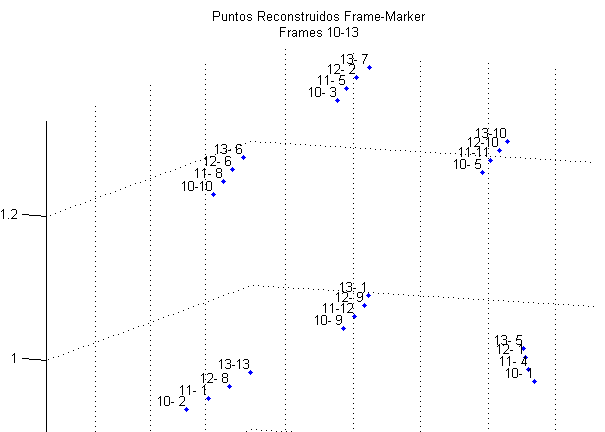
\includegraphics[scale=0.8]{img/Tracking/00_Salida_Reconstruccion}
\end{center}
\caption{Salida de Reconstrucción para 4 frames. La etiqueta para cada marcador es el indice en la reconstrucción para un determinado frame}
\label{reconstr_00}
\end{figure}

El procedimiento presentado \cite{herda}, es aplicar el tracking de partículas esbozado por Malik,Dracos,Papantoniou \cite{griegos} al seguimiento de marcadores. El mismo consiste en buscar el desplazamiento de un marcador desde el cuadro [f] al cuadro siguiente [f+1], sobre una ventana de cuatro cuadros. 

La hipótesis principal de este procedimiento, es que el muestreo del movimiento capturado  es suficiente para que el desplazamiento entre cuadros sea mínimo en distancia, y la idea para predecir y buscar el desplazamiento entre [f] y [f+1], es utilizar la información que se tiene de la secuencia entre [f-1] y [f], y utilizar una segunda proyección entre [f+1] y [f+2] para confirmar el enlace encontrado en el caso que exista mas de una posibilidad (figura \ref{herda_00}).

Para poder confirmar una trayectoria de 4 puntos, se debe cumplir que la misma presenta la menor variación de aceleración para la opción elegida entre todas las posibles, calculada como:

\begin{equation}
\begin{split}
\Delta{a}&= \left| \overrightarrow{a}_{[f+2][f+1][f]}-\overrightarrow{a}_{[f+1][f][f-1]} \right| \\
&= \left| \left(\overrightarrow{v}_{[f+2][f+1]}-\overrightarrow{v}_{[f+1][f]}\right)-\left(\overrightarrow{v}_{[f+1][f]}-\overrightarrow{v}_{[f][f-1]}\right) \right| \\
&= \left| x_{[f+2]} - 3.x_{[f+1]} + 3.x_{[f]} - x_{[f-1]} \right|\\
\end{split}
\label{track_var_acc}
\end{equation}

, donde $x_{[f+1]}$ a su vez, es aquel punto de [f+1] que mejor se aproxima al desplazamiento en frames anteriores, minimizando la ecuación \ref{track_acc} 

\begin{equation}
\begin{split}
\overrightarrow{v}_{[f+1][f]}& = \overrightarrow{v}_{[f][f-1]} \\
x_{[f+1]}-x_{[f]}& = x_{[f]}-x_{[f-1]} \\
\end{split}
\label{track_acc}
\end{equation}

\begin{figure}[hbt]
\begin{center}
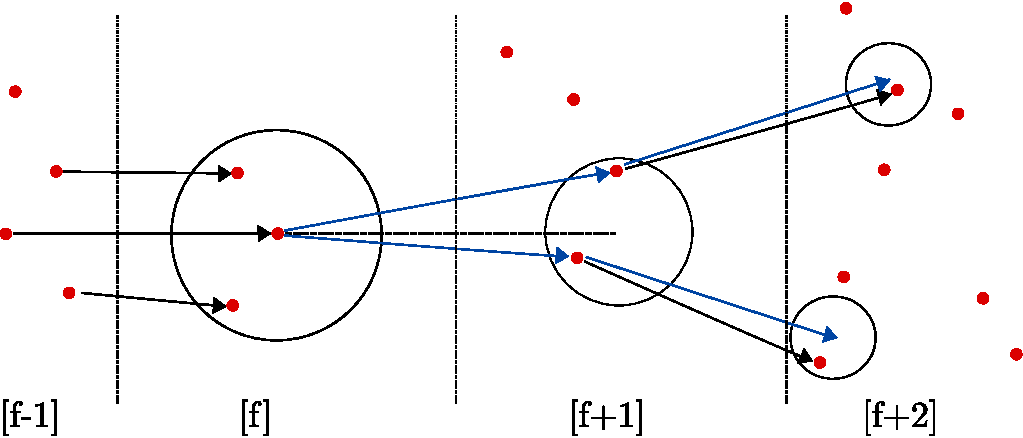
\includegraphics[scale=0.8]{img/Tracking/tracking-eps-converted-to.pdf}
\end{center}
\caption{Seguimiento en 4 frames, siendo [f] el frame actual que queremos seguir en [f+1]. La linea punteada es la traslación del movimiento previo, las lineas azules son las obtenidas buscando la mínima variación de aceleración para el punto elegido en [f+1]. De las dos posibles trayectorias, se elige aquella con menor variación de aceleración}
\label{herda_00}
\end{figure}

En su investigación\cite{herda}, Lorna Herda propone que realizar el seguimiento sobre la reconstrucción 3D presenta menos continuidad en las trayectorias , con respecto al seguimiento realizado sobre el conjunto de segmentación sumada a la proyección de los puntos reconstruidos 3D en cada vista 2D. Sin embargo, en nuestras pruebas, nos pareció mas coherente trabajar con el seguimiento en los puntos reconstruidos en 3D, ya que en caso de trayectorias que se cruzan en una vista 2D, son fácilmente separadas en 3D debido a la geometría. 

Adicionalmente, la reconstrucción fue implementada de forma distinta a la propuesta por Herda, si bien es posible obtener los puntos proyectados en cada vista, no cumplen el mismo rol. 

(Comparación Imagen de Tracking 2D, sobre 3D)

Finalmente, asumiendo que los puntos obtenidos directamente de las animaciones ,proyectados en cada cámara, son el mejor caso de puntos 2D, no presentaban grandes ventajas de trabajar el enlace en cada una de estas vistas 2D, sobre trabajar en 3D posteriormente a la reconstrucción, y no volver hacia atrás ya que la geometría entre vistas cumplió su cometido. Esto ultimo no se cumple para el caso que se evalúen medidas adicionales para robustecer la salida del tracking (ejemplo: validacion por visibilidad), como se estudiará en las conclusiones.

\subsection{Implementación}

Para un frame [f] y un marcador $m_{i}^{[f]}$, se desea encontrar en el frame [f+1] el marcador $m_{j}^{[f+1]}$ que continúe la trayectoria que se tiene hasta el momento, cumpliendo las ecuaciones de continuidad \ref{track_acc} y \ref{track_var_acc}. El elemento que traslada la informacion de un frame al siguiente y desde el anterior, es la matriz de enlaces, donde cada linea es un enlace, y cada enlace tiene los siguientes elementos:
\begin{equation}
\begin{bmatrix}
  m_{h}^{[f-1]} ,\quad m_{i}^{[f]} ,\quad m_{j}^{[f+1]} ,\quad m_{k}^{[f+2]} ,\quad \left|a_{[f-1][f][f+1]}\right| ,\quad \left|v_{[f][f+1]}\right|
\end{bmatrix}
\end{equation}

\subsubsection{Enlazado en régimen}



\subsubsection{Enlazado inicial y final}



\subsubsection{Inventario de trayectorias}



\subsection{Resultado y Analisis}


